\xiti
\begin{xiaotis}

\xiaoti{圆锥底面半径为 $r$,轴截面是直角三角形。求轴截面面积。}

\xiaoti{如图,圆柱的一个内接直三棱柱的一个侧面经过圆柱的轴。求证:这个棱柱其他两个侧面互相垂直。}

\begin{figure}[htbp]
    \centering
    \begin{minipage}[b]{4cm}
        \centering
        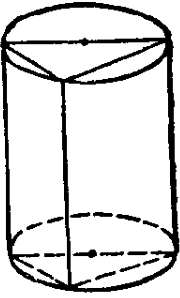
\includegraphics[width=3cm]{../pic/ltjh-ch2-xiti10-02.png}
        \caption*{(第 2 题)}
    \end{minipage}
    \qquad
    \begin{minipage}[b]{5cm}
        \centering
        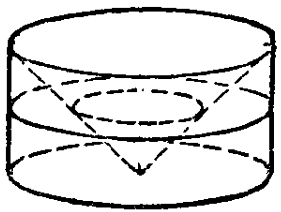
\includegraphics[width=4.5cm]{../pic/ltjh-ch2-xiti10-04.png}
        \caption*{(第 4 题)}
    \end{minipage}
    \qquad
    \begin{minipage}[b]{4cm}
        \centering
        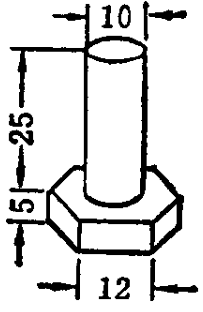
\includegraphics[width=3cm]{../pic/ltjh-ch2-xiti10-07.png}
        \caption*{(第 7 题)}
    \end{minipage}
\end{figure}

\xiaoti{经过高为 20 cm 的圆锥的顶点,与底面成 $45^\circ$ 二面角的平面把圆锥底面周长截去 $\exdfrac{1}{4}$。求截面面积。}

\xiaoti{从一个底面半径和高都是 $R$ 的圆柱中,挖去一个以圆柱上底面为底,下底面中心为顶点的圆锥,得到一个如图的几何体。
    如果用一个与圆柱下底面距离等于 $l$ 并且平行于底面的平面去截它,求截面面积。
}

\xiaoti{圆台的一个底面周长是另一个底面周长的3倍,轴截面的面积等于 $392\;\pflm$,母线与底面的夹角是 $45^\circ$,
    求这个圆台的高、母线长和两底面半径。
}

\xiaoti{已知圆柱的底面直径是 12 cm,高是 16 cm,内有一个以圆柱的底为底,另一个底的中心为顶点的圆锥。
    选择适当的比例尺,画出它们的直观图(不写画法)。
}

\xiaoti{要电镀螺杆(尺寸如图,单位: mm)。如果每平方米用锌 0.11 kg,电镀 100 个这样的螺杆需要多少锌?}

\xiaoti{一个圆锥的高是 10 cm,侧面展开图是半圆。求圆锥的侧面积。}

\xiaoti{用油漆涂 100 个圆台形水桶,桶口直径为 30 cm,桶底直径为 25 cm,母线长是 27.5 cm;
    已知每平方米需要油漆 150 g。 共需油漆多少 kg?
}

\xiaoti{圆锥的轴截面是正三角形。求证:它的侧面积是底面面积的 2 倍。}

\xiaoti{已知:圆台上、下底面面积是 $S'$、$S$,中截面面积为 $S_0$。
    求证: $2\sqrt{S_0} = \sqrt{S} + \sqrt{S'}$。
}

\begin{figure}[htbp]
    \centering
    \begin{minipage}[b]{7cm}
        \centering
        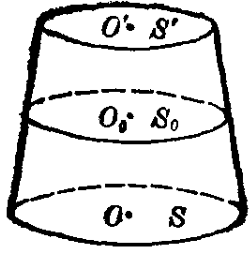
\includegraphics[width=4cm]{../pic/ltjh-ch2-xiti10-11.png}
        \caption*{(第 11 题)}
    \end{minipage}
    \qquad
    \begin{minipage}[b]{7cm}
        \centering
        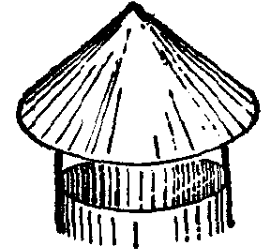
\includegraphics[width=4cm]{../pic/ltjh-ch2-xiti10-13.png}
        \caption*{(第 13 题)}
    \end{minipage}
\end{figure}

\xiaoti{已知圆台的上、下底面半径是 $r'$、$r$,它的侧面积等于两底面面积的和。求圆台的母线长。}

\xiaoti{如图,圆维形烟囱帽的底的半径是 40 cm,高是 30 cm。计算它的侧面展开图的圆心角和面积。}

\xiaoti{设圆台的上、下底面半径分别是 $r'$、$r$,母线长是 $l$。圆台侧面展开后所得的扇环的圆心角是 $\theta$。
    求证:$$ \theta = \dfrac{r - r'}{l} \cdot 360 (\text{度}) \juhao $$
}

\end{xiaotis}

